\documentclass[11pt,a4paper]{article}

\usepackage[margin=1in]{geometry}
\usepackage{amsmath,amssymb}
\usepackage{array,booktabs}
\usepackage{float}
\usepackage{graphicx}
\graphicspath{{../figures/}{figures/}{docs/submissions/figures/}}
\usepackage{fancyhdr}
\usepackage[hidelinks]{hyperref}

\setcounter{secnumdepth}{3}
\setcounter{tocdepth}{3}
\setlength{\parindent}{0pt}
\setlength{\parskip}{0.3em}
\setlength{\floatsep}{12pt plus 2pt minus 2pt}
\setlength{\textfloatsep}{12pt plus 2pt minus 2pt}
\setlength{\intextsep}{12pt plus 2pt minus 2pt}
\setlength{\abovecaptionskip}{6pt}
\setlength{\belowcaptionskip}{6pt}
\setlength{\tabcolsep}{8pt}
\renewcommand{\arraystretch}{1.18}

\pagestyle{fancy}
\setlength{\headheight}{14pt}
\fancyhf{}
\lhead{Deep Learning Laboratory}
\rhead{Lab Assignments 1 and 2}
\cfoot{\thepage}

\newcommand{\sigmoid}{\operatorname{sigmoid}}
\renewcommand{\thetable}{\arabic{section}.\arabic{table}}
\renewcommand{\thefigure}{\arabic{section}.\arabic{figure}}
\renewcommand{\theequation}{\arabic{section}.\arabic{equation}}
\renewcommand{\theHtable}{\arabic{section}.\arabic{table}}
\renewcommand{\theHfigure}{\arabic{section}.\arabic{figure}}
\renewcommand{\theHequation}{\arabic{section}.\arabic{equation}}

\begin{document}
\pagenumbering{gobble}

\begin{titlepage}
    \centering
    {\LARGE\bfseries Shiv Nadar University Chennai\par}
    \vspace{0.4cm}
    {\large M.Tech. Artificial Intelligence and Data Science\par}
    \vspace{0.2cm}
    {\large\bfseries Deep Learning Laboratory (26AI5705)\par}

    \vfill
    {\Huge\bfseries Deep Learning Laboratory Report\par}
    \vspace{0.5cm}
    {\Large Lab Assignments 1 and 2\par}

    \vfill
    {\large
    \renewcommand{\arraystretch}{1.35}
    \begin{tabular}{@{}rl@{}}
        \textbf{Submitted by:} & Mirthula (26120121) \\
                               & Karthikeyan M (26120004) \\
        \textbf{Submitted to:} & Prof. C. Chandra Sekhar \\
    \end{tabular}\par}
    \vfill
    {\large\bfseries Submission Date: 18 August 2026\par}
\end{titlepage}

\pagenumbering{roman}
\tableofcontents
\clearpage
\pagenumbering{arabic}

\section{Assignment 1}
\setcounter{table}{0}
\setcounter{figure}{0}
\setcounter{equation}{0}

\subsection{Objective}
The assignment covers vector comparison, activation functions and derivatives, one feedforward/backpropagation step, and feature normalization. MATLAB source files are provided in the \texttt{lab1} folder.

\subsection{Vector Distance and Similarity}

For vectors $\mathbf{u},\mathbf{v}\in\mathbb{R}^{n}$,
\begin{align}
    d(\mathbf{u},\mathbf{v})
    &=\sqrt{\sum_{i=1}^{n}(u_i-v_i)^2}, \\
    \cos(\mathbf{u},\mathbf{v})
    &=\frac{\mathbf{u}^{T}\mathbf{v}}
    {\lVert\mathbf{u}\rVert_2\lVert\mathbf{v}\rVert_2}.
\end{align}

Using
\[
\mathbf{x}=[3,-4,6,-1],\quad
\mathbf{y}=[-2,5,8,-3],\quad
\mathbf{z}=[5,3,-1,-4],
\]
the results are:

\begin{table}[H]
\centering
\caption{Vector comparison results.}
\begin{tabular}{lcc}
\toprule
Pair & Euclidean distance & Cosine similarity \\
\midrule
$\mathbf{x},\mathbf{y}$ & $10.6771$ & $0.3144$ \\
$\mathbf{x},\mathbf{z}$ & $10.5357$ & $0.0178$ \\
\bottomrule
\end{tabular}
\end{table}

The first pair has the larger angular similarity. The second pair is almost orthogonal.

\subsection{Activation Functions}

\begin{table}[H]
\centering
\small
\caption{Activation functions used in the assignment.}
\begin{tabular}{>{\raggedright\arraybackslash}p{2.3cm}p{4.8cm}p{4.7cm}}
\toprule
Function & $f(x)$ & Output range \\
\midrule
Sigmoid & $\displaystyle \frac{1}{1+e^{-\beta x}}$ & $(0,1)$ \\
Tanh & $\tanh(\beta x)$ & $(-1,1)$ \\
ReLU & $\max(0,x)$ & $[0,\infty)$ \\
Softplus & $\ln(1+e^x)$ & $(0,\infty)$ \\
Leaky ReLU & $\begin{cases}\delta x,&x<0\\x,&x\geq0\end{cases}$ & $(-\infty,\infty)$ for $\delta>0$ \\
Swish & $x\,\sigmoid(\beta x)$ & approximately $[-0.278,\infty)$ for $\beta=1$ \\
\bottomrule
\end{tabular}
\end{table}

\begin{figure}[H]
    \centering
    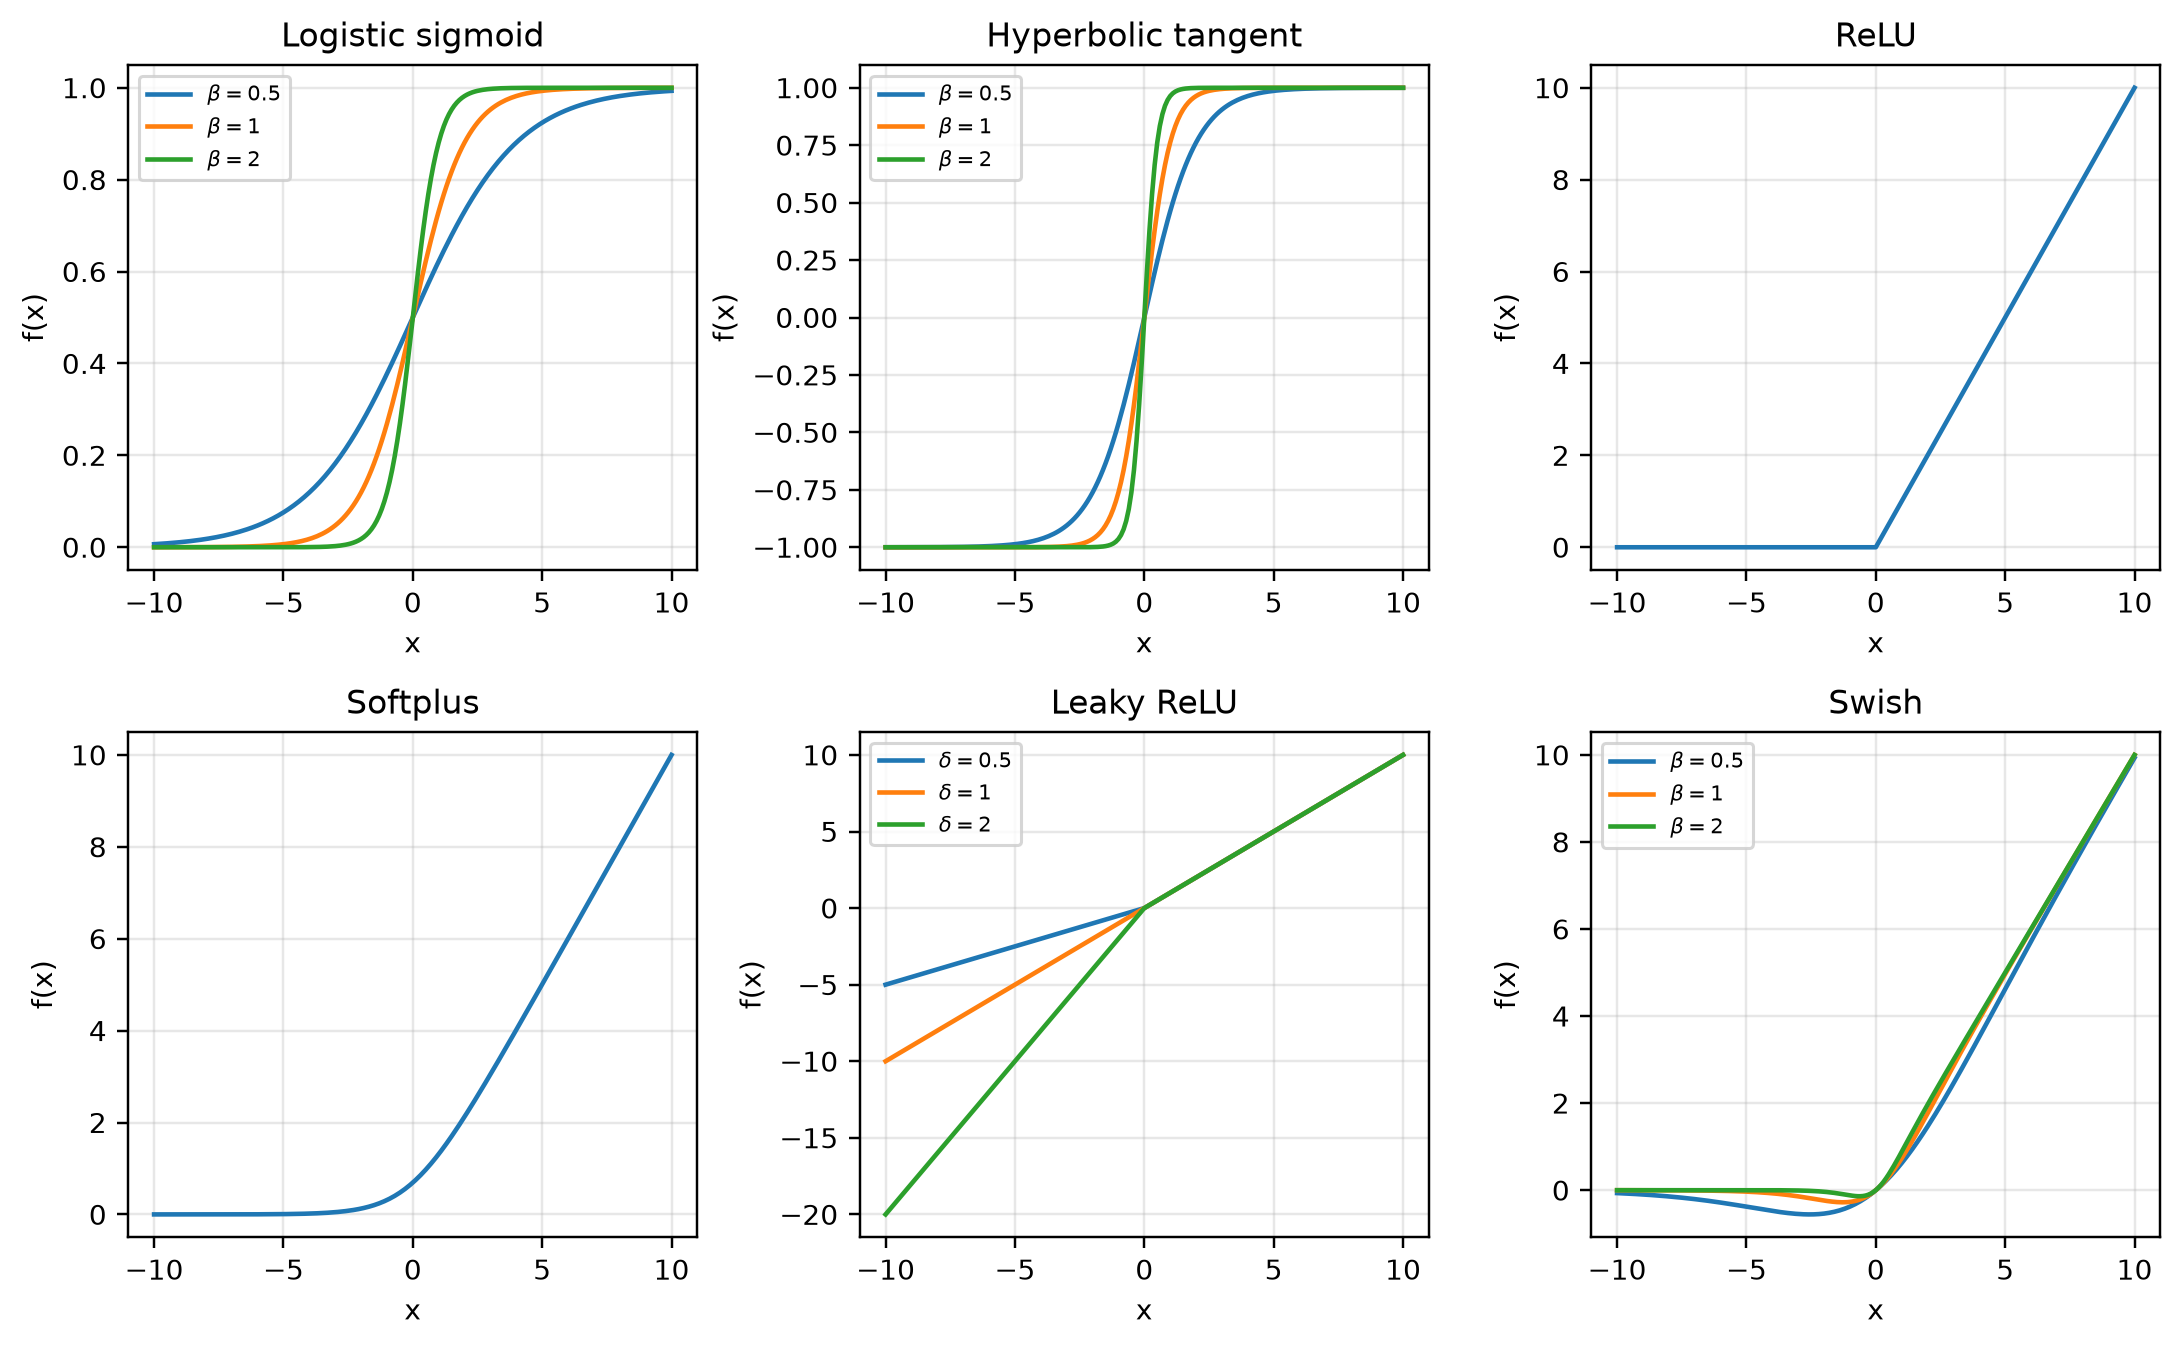
\includegraphics[width=\textwidth]{Lab1/activation_functions.png}
    \caption{Activation functions for the required $\beta$ and $\delta$ values.}
\end{figure}

Increasing $\beta$ makes sigmoid and tanh steeper. ReLU is piecewise linear, Softplus is its smooth approximation, and Swish is smooth and non-monotonic.

\subsection{Activation Derivatives}

\begin{table}[H]
\centering
\small
\caption{Analytical derivatives. Values at $x=0$ for piecewise functions may be assigned by convention.}
\begin{tabular}{lp{9.2cm}}
\toprule
Function & $f'(x)$ \\
\midrule
Sigmoid & $\beta\sigma(\beta x)\bigl(1-\sigma(\beta x)\bigr)$ \\
Tanh & $\beta\bigl(1-\tanh^2(\beta x)\bigr)$ \\
ReLU & $0$ for $x<0$; $1$ for $x>0$ \\
Softplus & $\sigma(x)$ \\
Leaky ReLU & $\delta$ for $x<0$; $1$ for $x>0$ \\
Swish & $\sigma(\beta x)+\beta x\sigma(\beta x)\bigl(1-\sigma(\beta x)\bigr)$ \\
\bottomrule
\end{tabular}
\end{table}

\begin{figure}[H]
    \centering
    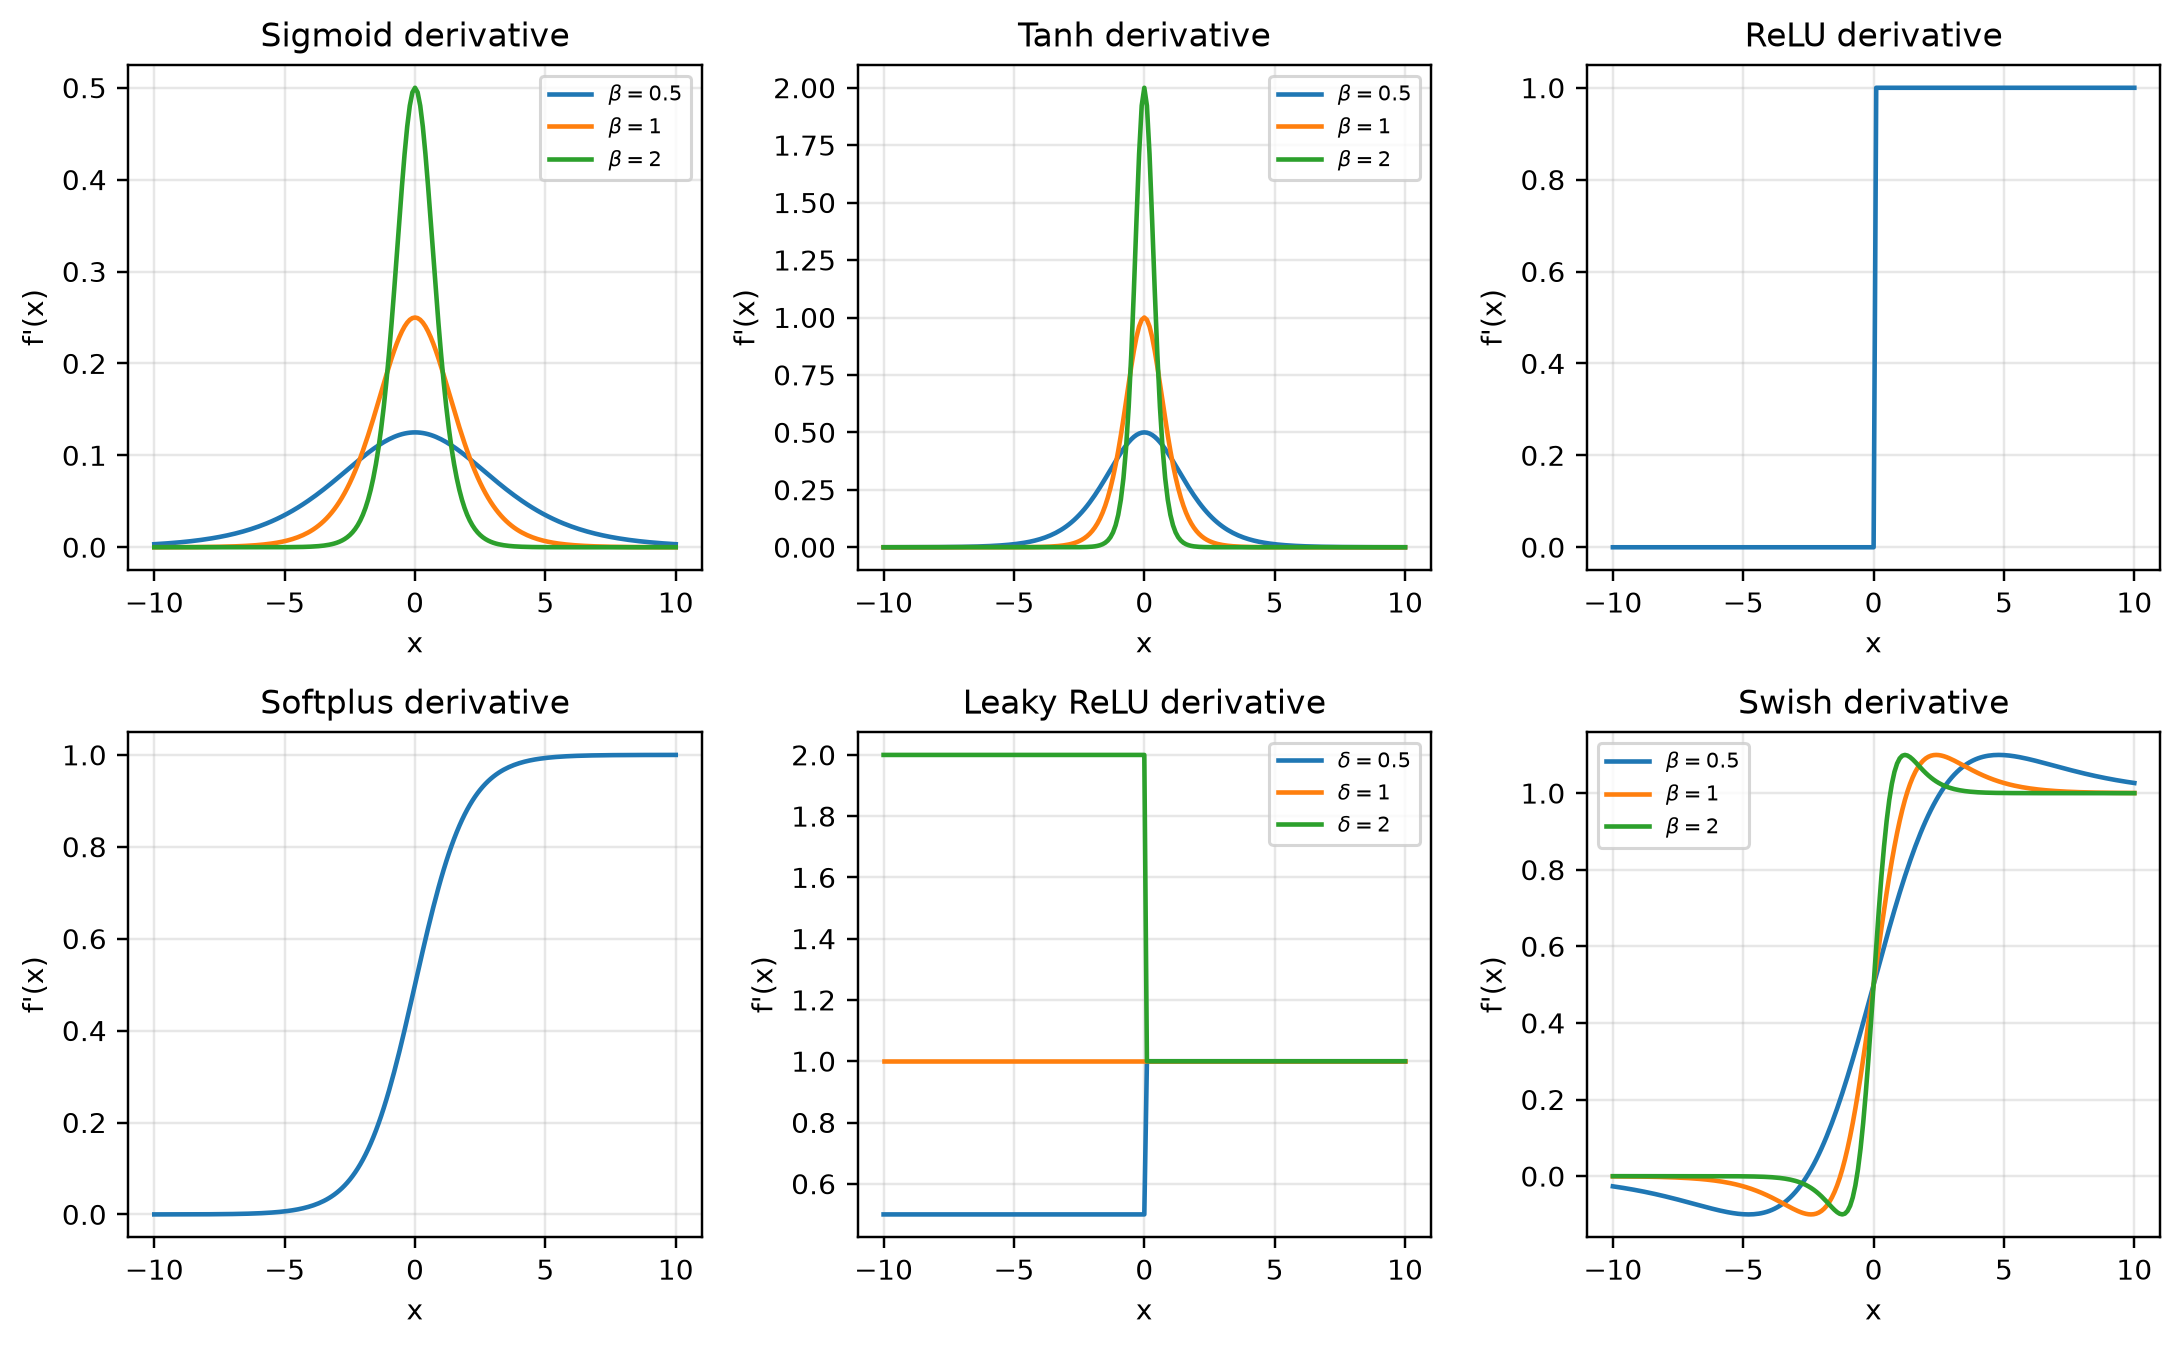
\includegraphics[width=\textwidth]{Lab1/activation_derivatives.png}
    \caption{Derivatives of the six activation functions.}
\end{figure}

\subsection{Feedforward and Backpropagation}

The network contains two inputs, four tanh hidden nodes, and three sigmoid output nodes. The Class 2 target is
\[
\mathbf{x}=[2.5,-4.3],\qquad \mathbf{t}=[0,1,0],\qquad \eta=0.9.
\]

\subsubsection{Forward pass}
\begin{align}
    \mathbf{a}^{h} &= \mathbf{x}W_h+\mathbf{b}_h, &
    \mathbf{h} &= \tanh(\mathbf{a}^{h}),\\
    \mathbf{a}^{o} &= \mathbf{h}W_o+\mathbf{b}_o, &
    \mathbf{y} &= \sigmoid(\mathbf{a}^{o}),\\
    E &= \frac{1}{2}\sum_{k=1}^{3}(t_k-y_k)^2.
\end{align}

\begin{align*}
\mathbf{a}^{h}&=[-5.0900,\ 3.8600,\ 0.4100,\ -7.6700],\\
\mathbf{h}&=[-0.999924,\ 0.999113,\ 0.388473,\ -1.000000],\\
\mathbf{a}^{o}&=[2.010487,\ 1.255786,\ 1.775349],\\
\mathbf{y}&=[0.881894,\ 0.778300,\ 0.855122],\\
E&=0.779060.
\end{align*}

\subsubsection{Local gradients}
\begin{align}
    \boldsymbol{\delta}^{o}
    &=(\mathbf{t}-\mathbf{y})\odot\mathbf{y}\odot(1-\mathbf{y}),\\
    \boldsymbol{\delta}^{h}
    &=(\boldsymbol{\delta}^{o}W_o^T)\odot(1-\mathbf{h}^2).
\end{align}

\begin{align*}
\boldsymbol{\delta}^{o}
&=[-0.091856,\ 0.038254,\ -0.105940],\\
\boldsymbol{\delta}^{h}
&=[2.8591\!\times\!10^{-5},\ -3.0012\!\times\!10^{-4},\ -0.324714,\ -2.5054\!\times\!10^{-7}].
\end{align*}

\subsubsection{Parameter changes}
\begin{align}
    \Delta W_o &= \eta\,\mathbf{h}^{T}\boldsymbol{\delta}^{o}, &
    \Delta\mathbf{b}_o &= \eta\boldsymbol{\delta}^{o},\\
    \Delta W_h &= \eta\,\mathbf{x}^{T}\boldsymbol{\delta}^{h}, &
    \Delta\mathbf{b}_h &= \eta\boldsymbol{\delta}^{h}.
\end{align}

\[
\Delta W_o=\begin{bmatrix}
 0.082664&-0.034426& 0.095339\\
-0.082597& 0.034398&-0.095261\\
-0.032115& 0.013375&-0.037039\\
 0.082670&-0.034429& 0.095346
\end{bmatrix},\quad
\Delta\mathbf{b}_o=[-0.082670,\ 0.034429,\ -0.095346].
\]

\[
\Delta W_h=\begin{bmatrix}
 0.000064&-0.000675&-0.730605&-0.000001\\
-0.000111& 0.001161& 1.256641& 0.000001
\end{bmatrix},
\]
\[
\Delta\mathbf{b}_h=[0.000026,\ -0.000270,\ -0.292242,\ -0.000000].
\]

The updated parameters are obtained using $W^{\text{new}}=W+\Delta W$ and $\mathbf{b}^{\text{new}}=\mathbf{b}+\Delta\mathbf{b}$.

\subsection{Feature Normalization}

Min-max and mean-variance normalization are
\begin{align}
    x_i' &= \frac{x_i-x_{\min}}{x_{\max}-x_{\min}},\\
    z_i &= \frac{x_i-\bar{x}}{s}.
\end{align}
MATLAB's sample standard deviation is used: $\bar{x}_1=1.3$, $s_1=4.5717$, $\bar{x}_2=2.1$, and $s_2=9.9605$.

\begin{table}[H]
\centering
\scriptsize
\caption{Normalized feature values.}
\begin{tabular}{rrrrrr}
\toprule
$x_1$ & $x_2$ & Min-max $x_1$ & Min-max $x_2$ & Standard $x_1$ & Standard $x_2$\\
\midrule
-2& 12&0.2857&0.8929&-0.7218& 0.9939\\
 5& 15&0.7857&1.0000& 0.8093& 1.2951\\
-3&-13&0.2143&0.0000&-0.9406&-1.5160\\
 7& -6&0.9286&0.2500& 1.2468&-0.8132\\
 4&  4&0.7143&0.6071& 0.5906& 0.1908\\
-1& -7&0.3571&0.2143&-0.5031&-0.9136\\
 8& 13&1.0000&0.9286& 1.4656& 1.0943\\
-6& -2&0.0000&0.3929&-1.5968&-0.4116\\
 0& 10&0.4286&0.8214&-0.2844& 0.7931\\
 1& -5&0.5000&0.2857&-0.0656&-0.7128\\
\bottomrule
\end{tabular}
\end{table}

\subsection{Conclusion}
The calculations verify the vector metrics, activation derivatives, one generalized-delta update, and both normalization methods. The figures show how the activation parameters control slope and gradient magnitude.

\clearpage
\section{Assignment 2}
\setcounter{table}{0}
\setcounter{figure}{0}
\setcounter{equation}{0}

\subsection{Objective}
The task is to classify two nonlinearly separable classes using two hidden-layer networks. The 6-4 and 12-8 configurations are compared using validation accuracy, and the selected model is evaluated on the test set.

\subsection{Dataset and Preprocessing}

Dataset 1 contains two features and a binary label.

\begin{table}[H]
\centering
\caption{Dataset splits.}
\begin{tabular}{lrr}
\toprule
Split & Examples & Use \\
\midrule
Training & 1123 & Weight updates \\
Validation & 317 & Configuration selection \\
Test & 160 & Final evaluation \\
\bottomrule
\end{tabular}
\end{table}

Each feature is standardized using training statistics only:
\begin{equation}
    x_j'=\frac{x_j-\mu_j^{\text{train}}}{s_j^{\text{train}}}.
\end{equation}
This prevents validation and test information from entering training.

\subsection{Network Model}

\begin{table}[H]
\centering
\caption{Network configurations.}
\begin{tabular}{lcccc}
\toprule
Configuration & Inputs & Hidden layer 1 & Hidden layer 2 & Output \\
\midrule
6-4 & 2 & 6 & 4 & 1 \\
12-8 & 2 & 12 & 8 & 1 \\
\bottomrule
\end{tabular}
\end{table}

For one input pattern $\mathbf{x}$,
\begin{align}
    \mathbf{h}_1 &= \tanh(W_1\mathbf{x}+\mathbf{b}_1),\\
    \mathbf{h}_2 &= \tanh(W_2\mathbf{h}_1+\mathbf{b}_2),\\
    \hat{y} &= \sigmoid(W_3\mathbf{h}_2+b_3).
\end{align}

The activations use $\beta=1$. Binary cross-entropy is
\begin{equation}
    E=-\frac{1}{N}\sum_{i=1}^{N}
    \left[y_i\ln(\hat{y}_i)+(1-y_i)\ln(1-\hat{y}_i)\right].
\end{equation}

\subsection{Training Method}

Pattern-mode learning updates the parameters after every example. SGD uses the required learning rate and momentum:
\begin{equation}
    \Delta\theta_t=-\eta\nabla_{\theta}E_t+\alpha\Delta\theta_{t-1},
    \qquad \eta=0.8,\quad \alpha=0.9.
\end{equation}

The patterns are shuffled each epoch, and the seed is reset before each configuration. Gradient norm clipping at $0.1$ limits unstable single-pattern updates. Training stops after three consecutive epochs satisfy
\begin{equation}
    \left|E_{\text{train}}^{(e)}-E_{\text{train}}^{(e-1)}\right|<0.01.
\end{equation}
The three-epoch check avoids stopping because of one noisy pattern-mode epoch.

\subsection{Results}

\subsubsection{Configuration 1: 6-4}

Training stopped after 86 epochs. The final training accuracy was $97.60\%$ and validation accuracy was $96.21\%$.

\begin{figure}[H]
\centering
\begin{minipage}[t]{0.49\textwidth}
    \centering
    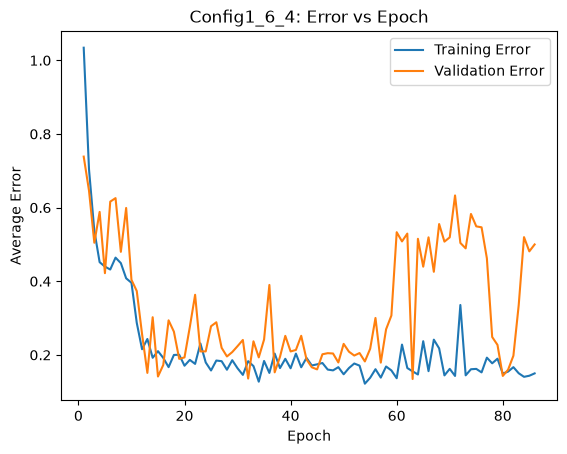
\includegraphics[width=\linewidth]{Lab2/config1_error_vs_epoch.png}
    \small (a) Training and validation error
\end{minipage}
\hfill
\begin{minipage}[t]{0.49\textwidth}
    \centering
    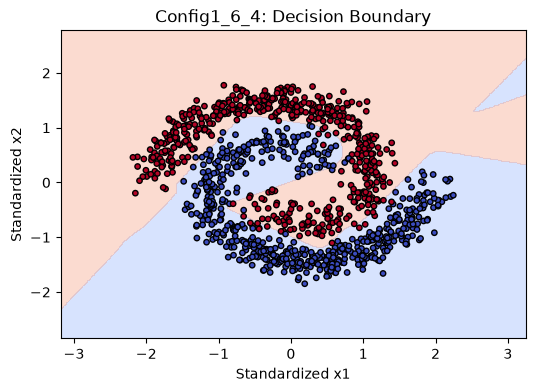
\includegraphics[width=\linewidth]{Lab2/config1_decision_boundary.png}
    \small (b) Decision boundary
\end{minipage}
\caption{Results for the 6-4 configuration.}
\end{figure}

\subsubsection{Configuration 2: 12-8}

Training stopped after 29 epochs. The final training accuracy was $98.13\%$ and validation accuracy was $97.79\%$.

\begin{figure}[H]
\centering
\begin{minipage}[t]{0.49\textwidth}
    \centering
    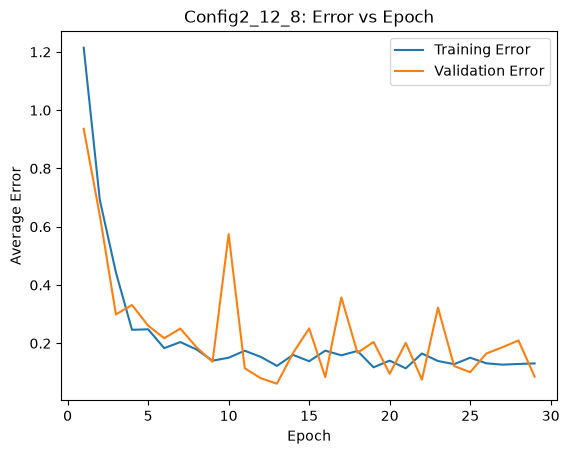
\includegraphics[width=\linewidth]{Lab2/config2_error_vs_epoch.png}
    \small (a) Training and validation error
\end{minipage}
\hfill
\begin{minipage}[t]{0.49\textwidth}
    \centering
    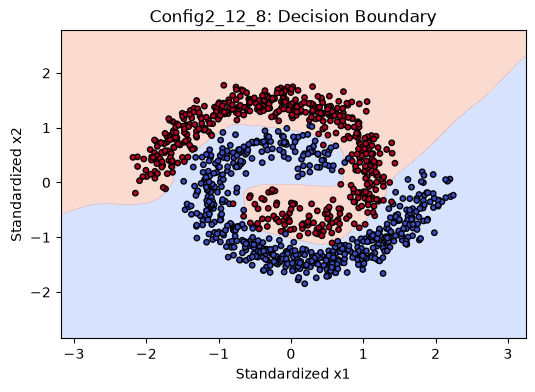
\includegraphics[width=\linewidth]{Lab2/config2_decision_boundary.png}
    \small (b) Decision boundary
\end{minipage}
\caption{Results for the 12-8 configuration.}
\end{figure}

\subsubsection{Validation Selection}

\begin{table}[H]
\centering
\caption{Accuracy comparison.}
\begin{tabular}{lrrr}
\toprule
Configuration & Stop epoch & Training accuracy & Validation accuracy \\
\midrule
6-4 & 86 & $97.60\%$ & $96.21\%$ \\
12-8 & 29 & $98.13\%$ & $97.79\%$ \\
\bottomrule
\end{tabular}
\end{table}

The 12-8 configuration has the higher validation accuracy and is selected. Its test accuracy is
\begin{equation}
    \boxed{98.75\%}.
\end{equation}

\subsection{Discussion}

The error curves fluctuate because pattern-mode updates use one shuffled example at a time with a large learning rate and momentum. The training-validation accuracy gaps are only $1.39$ and $0.34$ percentage points, so there is no strong evidence of overfitting. Both decision plots capture the nonlinear spiral-like class boundary.

\subsection{Conclusion}

Both networks learned the nonlinear classes. Validation accuracy selected the 12-8 model, which achieved $98.75\%$ accuracy on the unseen test data.

\end{document}
